
\renewcommand{\summarizedlecture}{11 }

%
%
%

\begin{frame}{Lecture \summarizedlecture - \lecturesummarytitle}

\begin{columns}
  \begin{column}{0.25\textwidth}
    \begin{center}
       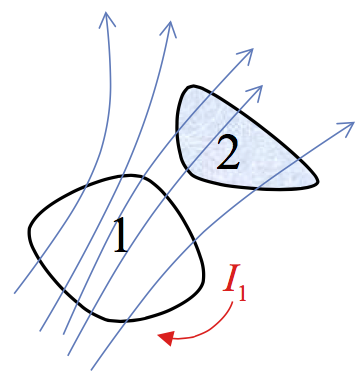
\includegraphics[width=0.90\textwidth]{./images/schematics/mutual_inductance_1.png}\\
     \end{center}
  \end{column}
  \begin{column}{0.75\textwidth}
  {\scriptsize
       The flux through the surface of loop 2, of the magnetic field $\vec{B}_1$
       produced by the current $I_1$ in loop 1 is:
       \begin{equation*}
            \Phi_2 = M_{21}  I_1
       \end{equation*}
       The constant of proportionality ($M_{21}$) is known as {\bf mutual inductance}.\\
       It is:
       \begin{itemize}
           \item purely geometrical, and
           \item unchanged if one switches the roles of loop 1 and 2.\\
       \end{itemize}
   }
  \end{column}
\end{columns}

\vspace{0.4cm}

{\scriptsize
       So \underline{whatever} the shapes and positions of the loops,
       the flux through loop 2 when we run a current I around loop 1 is
       identical to the flux through loop 1 when we run the same current around loop 2.
      \begin{equation*}
            M_{21}  = M_{12} = M
       \end{equation*}

        The SI unit of the mutual inductance is the {Henry} (H)
        \begin{itemize}
              \item A derived unit.
              \item 1 H = $\displaystyle \frac{Wb}{A}$ = $\displaystyle \frac{V \cdot s}{A}$
        \end{itemize}
}
\end{frame}

%
%
%

\begin{frame}{Lecture \summarizedlecture - \lecturesummarytitle (cont'd)}

{ \scriptsize
We also considered what happens if the current varies with time.
\begin{itemize}
  { \scriptsize
   \item  time-varying current $\rightarrow$ time-varying magnetic field
   \item  time-varying magnetic field $\rightarrow$  time-varying flux.
   \item  time-varying flux $\rightarrow$ EMF (Faraday's law)
  }
\end{itemize}

\vspace{0.3cm}

{\bf A change in current flow in a conductor induces a voltage (EMF)}
\vspace{0.2cm}
\begin{itemize}
  { \scriptsize
   \item in the same conductor (self-inductance): \\
             $\displaystyle \mathcal{E} = - L \frac{dI}{dt}$
   \vspace{0.2cm}
   \item and in neighbouring conductors (mutual inductance):\\
            $\displaystyle \mathcal{E}_{neighbouring\;loop} = - M \frac{dI}{dt}$
  }
\end{itemize}

\vspace{0.2cm}

In both cases the inductance (mutual or self) is the {\bf constant of proportionality}
between the EMF developed and the rate of current change.

\vspace{0.2cm}

We also studied the solenoid and its inductance per unit length (far from the ends of the solenoid) is:
\begin{equation*}
  L =  \mu_0 \cdot n^2 \cdot A
\end{equation*}
where $A$ is the area of each winding, and $n$ the number of turns per unit length.
}
\end{frame}

%
%
%

\begin{frame}{Lecture \summarizedlecture - \lecturesummarytitle (cont'd)}

Then we studied DC circuits with resistors, capacitors and inductors.

\begin{columns}
  \begin{column}{0.40\textwidth}
    \begin{center}
         \begin{circuitikz} [scale=0.7]
            \draw
                 (0,0) to[battery=$\varepsilon$] (0,2)
                         to[short, -o] (0.75, 2.0);
             \draw[very thick]
                  (0.78,2.0)--(1.22,2.0);
             \draw
                  (1.25, 2.0) to [short, o-] (2,2)
                                   to[R=$R$, i=$I$] (2,0)
                                   to[L=$L$] (0,0);
         \end{circuitikz}
     \end{center}
  \end{column}
  \begin{column}{0.60\textwidth}
   {\scriptsize
       We studied an RL circuit and we saw that its behaviour is determined
      by the following differential equation:
       \begin{equation*}
              \mathcal{E} -L \cdot \frac{dI}{dt} = I \cdot R
      \end{equation*}
   }
  \end{column}
\end{columns}

\begin{columns}
  \begin{column}{0.40\textwidth}
       \begin{center}
           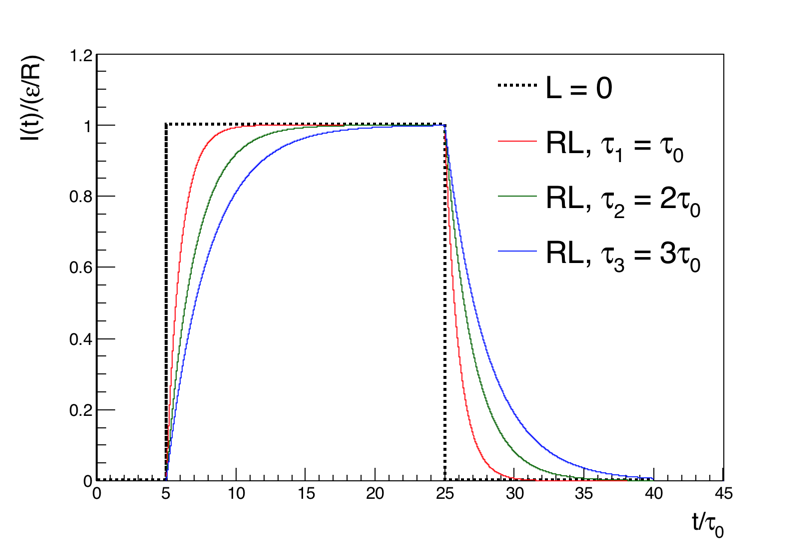
\includegraphics[width=0.95\textwidth]{./images/misc/ItRL_2.png}\\
       \end{center}
  \end{column}
  \begin{column}{0.60\textwidth}
  {\scriptsize
      We solved that equation which gave as the following solutions for the
      current after connecting or disconnecting the EMF:
      \begin{equation*}
       {\color{magenta}
            I(t) = \frac{\mathcal{E}}{R} \Big(1 - exp^{-\frac{t}{\tau}} \Big)
       }
       \;\;\; and \;\;\;
      {\color{magenta}
           I(t) = \frac{\mathcal{E}}{R} \cdot exp^{-\frac{t}{\tau}}
      }
      \end{equation*}
      Note that times are measured from the corresponding point of
      connecting or disconnecting the EMF.\\
  }
  \end{column}
\end{columns}

{\scriptsize
  {\bf Inductance is a kind of inertia in the circuit}. \\
  \vspace{0.1cm}
  So it is {\bf no longer possible to just change the current instantaneously} (as when L=0).
}
\end{frame}

%
%
%

\begin{frame}{Lecture \summarizedlecture - \lecturesummarytitle (cont'd)}

{ \scriptsize
We saw that the energy stored in the magnetic field of an inductor is: $\displaystyle U_B = \frac{1}{2} LI^2$.\\

\vspace{0.2cm}
Then we studied LC and RLC circuits both qualitatively and quantitatively:
\begin{columns}
  \begin{column}{0.50\textwidth}
     \begin{center}
         \begin{circuitikz} [scale=0.8]
            \draw
                 (0,0) to[battery=$\varepsilon$] (0,2) to[short, -o] (0.75, 2.0);
             \draw[very thick]
                  (0.78,2.0)--(1.18,2.3);
             \draw
                  (1.25, 2.0) to [short, o-] (2,2) to[C=$C$] (2,0)--(0,0);
              \draw
                  (2,2)--(4,2) to[L=$L$,i=$I$] (4,0) -- (2,0);
         \end{circuitikz}
     \end{center}
  \end{column}
  \begin{column}{0.50\textwidth}
     \begin{center}
         \begin{circuitikz} [scale=0.8]
            \draw
                 (0,0) to[battery=$\varepsilon$] (0,2) to[short, -o] (0.75, 2.0);
             \draw[very thick]
                  (0.78,2.0)--(1.18,2.3);
             \draw
                  (1.25, 2.0) to [short, o-] (2,2) to[C=$C$] (2,0)--(0,0);
              \draw
                  (2,2) to[R=$R$]  (4,2) to[L=$L$,i=$I$] (4,0) -- (2,0);
         \end{circuitikz}
     \end{center}
  \end{column}
\end{columns}

\vspace{0.2cm}

RL and RLC are described by the following differential equation (with R=0 for LC):
\begin{equation*}
          L \frac{d^2q}{dt^2} + R \frac{dq}{dt} + \frac{1}{C}q = 0
\end{equation*}

\vspace{0.2cm}
\begin{itemize}
\item
 Which saw that for R=0 we have undamped oscillations of charge, current and voltage and
that the stored energy is transferred fully between the capacitor (electric field) and the
inductor (magnetic field).
\item
For R$\ne$0 we have damped oscillations as, on every iteration, a fraction of the available energy is
converted to heat.
\end{itemize}
}

\end{frame}
